\documentclass{article}

% --- Grundlegende Dokumenteneinstellungen ---
\usepackage[utf8]{inputenc}       % Kodierung (bei modernem LuaLaTeX/XeLaTeX nicht mehr nötig)
\usepackage[T1]{fontenc}          % Korrekte Trennung von Wörtern mit Umlauten
\usepackage[ngerman]{babel}       % Deutsche Rechtschreibung und Bezeichnungen
\usepackage{geometry}             % Seitenränder einstellen
\usepackage{parskip}              % Absätze durch Abstand statt Einrückung trennen

% --- Grafik & Design ---
\usepackage{graphicx}             % Einbinden von Bildern
\usepackage{xcolor}               % Farben nutzen
\usepackage{float}                % Bessere Platzierung von Bildern ([H])
\usepackage{tikz}                 % Zeichnungen direkt in LaTeX
\usepackage{tcolorbox}            % Schicke Boxen für Hervorhebungen

% --- Mathe & Symbole ---
\usepackage{amsmath}              % Standard für mathematische Formeln
\usepackage{seqsplit}             % Lange Zeichenfolgen (z.B. DNA) umbrechen

% --- Programmierung & Code ---
\usepackage{listings}             % Quellcode-Darstellung
% --- Farben für die Code-Boxen definieren ---
\definecolor{codebackground}{rgb}{0.95, 0.95, 0.96}
\definecolor{codeframe}{rgb}{0.75, 0.75, 0.8}

% --- Globale Einstellungen für das listings-Paket ---
\lstset{
    backgroundcolor=\color{codebackground}, % Heller Hintergrund
    frame=single,                           % Ein einfacher Rahmen um den Code
    rulecolor=\color{codeframe},            % Farbe des Rahmens
    basicstyle=\ttfamily\small,             % Schriftart und Größe
    breaklines=true,                        % Zeilenumbrüche aktivieren
    captionpos=b,                           % Bildunterschrift (Caption) nach unten (bottom)
    keepspaces=true,                        % Leerzeichen exakt beibehalten
    numbers=left,                           % Zeilennummern auf der linken Seite
    numberstyle=\tiny\color{gray},          % Stil der Zeilennummern
    xleftmargin=2em,                        % Abstand zum linken Rand (Platz für Nummern)
    framexleftmargin=1.5em                  % Rahmen zieht sich um die Nummern
}



% --- Verweise & Hyperlinks (Immer als letztes laden!) ---
\usepackage{hyperref}
\hypersetup{
    colorlinks=true, 
    urlcolor=blue,
    linkcolor=black               % Optional: interne Links schwarz lassen
}


\begin{document}

\begin{titlepage}
    \centering

   

    % Hochschulkontext
    \textbf{Fachbereich Technik – Studiengang Informatik}
    \vspace{2.5cm}

    % Titel
    {\Huge\bfseries Aufgabe 2 \par}
    \vspace{1cm}
    {\Large zum Modul\\[0.3cm]
    \textit{Parralele und verteilte Systeme}\par}
    \vspace{1cm}
    {\large Sommersemester 2026\par}

    \vfill

    % Persönliche Angaben
    \begin{flushleft}
    \textbf{Gruppe: B2}
    \end{flushleft}
\end{titlepage}





\tableofcontents

\newpage




% --- Punkt 1 (Platzhalter, falls benötigt) ---
\section{Aufgabe 1}
In dieser Aufgabe geht es darum einen Verkaufsautomaten in mCRL2 zu spezifizieren. Dazu wurden zunächst die Münzen und deren Werte spezifiziert. Diese gehen, wie in Listing \ref{lst:coins} zu erkennen ist, von fünf Cent bis zu einem Euro.

\begin{lstlisting}[caption={Definition der Münzen},label={lst:coins}]
% Definition of the coins
%
sort
  Coin = struct _5c | _10c | _20c | _50c | Euro;

map
  value: Coin  -> Int;    % the value of a coin as an integer

eqn
  value(_5c) = 5;
  value(_10c) = 10;
  value(_20c) = 20;
  value(_50c) = 50;
  value(Euro) = 100;
\end{lstlisting}

Anschließend wurden die Preise der Produkte definiert. Diese sind je nach Produkt unterschiedlich und sind in Listing \ref{lst:produkte} zu erkennen.

\begin{lstlisting}[caption={Definition der Produkte},label={lst:produkte}]
% Definition of the products
%
sort
  Product = struct tea | coffee | cake | apple;

map
  price: Product  -> Int; % the price of a product as an integer

eqn
  price(tea) = 10;
  price(coffee) = 25;
  price(cake) = 60;
  price(apple) = 80;	
\end{lstlisting}

Als nächstes wurden die gültigen Funktionen des Automaten definiert. Dabei handelt es sich wie in dem Listing \ref{lst:actions} zu erkennen um das akzeptieren von Münzen, dem ausgeben von münzen, dem Anbieten und servieren von Produkten und zum Schluss dem zurückgeben des Wechselgeldes.

\begin{lstlisting}[caption={Definition der Funktionen},label={lst:actions}]
% Definition of the actions
%
act
  accept: Coin;        % accept a coin inserted into the machine    
  return: Coin;        % returns change
  offer: Product;      % offer the possibility to order a certain product
  serve: Product;      % serve a certain product
  returnChange: Int;   % request to return the current credit as  change
\end{lstlisting}

Das Verhalten des Automaten wird in einem Prozess beschrieben. Im Hauptprozess können drei verschiedene Sachen gemacht werden. 

\begin{enumerate}
	\item{Münze einwerfen und Guthaben erhöhen (wenn unter 200)}
	\item{Produkt anbieten (wenn Guthaben genügt)}
	\item{Wechselgeld anfordern (Falls noch Guthaben da ist)}
\end{enumerate}

Der Hauptprozess ist in Listing \ref{lst:vm} dargestellt. Dabei wurde wie angefordert der sum Operator verwendet. Zudem wurden Überprüfungen eingebaut, um zu verhindern, dass bei einem Guthaben von über 200 das Guthaben weiter erhöht werden kann und nur Produkte angeboten werden, für die ausreichend Guthaben vorhanden ist. 

\begin{lstlisting}[caption={Hauptprozess des Automaten},label={lst:vm}]
VM(credit : Int) =
	% 1. Insert a coin and add the value to the credit (only if the credit is below 200)
	sum c: Coin . (credit < 200) -> accept(c) . VM(credit + value(c))
	+
	% 2. Offer a product, but only if the credit is high enough -> serve -> reduce credit
	sum p: Product . (credit >= price(p)) -> offer(p) . serve(p) . VM(credit - price(p))
	+
	% 3. Initiate change return if there is a balance
	(credit > 0) -> returnChange(credit) . ReturnChange(credit)
;
\end{lstlisting}

Das Wechselgeld anfordern befindet sich in einem Unterprozess. Dieser ist in Listing \ref{lst:wechselgeld} dargestellt. Die Strategie in dabei ist es zu schauen, wie hoch das aktuelle Guthaben ist und abhängig davon die größte Münze auszugeben. Nachdem sich dadurch das Guthaben verringert wurde, ruft sich der Prozess rekursiv mit dem neuen Guthaben auf.

\begin{lstlisting}[caption={Prozess für die Rückgabe des Wechselgeldes},label={lst:wechselgeld}]
% Return the credit from high to low coins
ReturnChange(credit : Int) =
	(credit >= 100) -> return(Euro) . ReturnChange(credit - 100)
	+
	(credit >= 50 && credit < 100) -> return(_50c) . ReturnChange(credit - 50)
	+
	(credit >= 20 && credit < 50) -> return(_20c) . ReturnChange(credit - 20)
	+
	(credit >= 10 && credit < 20) -> return(_10c) . ReturnChange(credit - 10)
	+
	(credit >= 5 && credit < 10) -> return(_5c) . ReturnChange(credit - 5)
	+
	(credit == 0) -> VM(0)
;
\end{lstlisting}



%Ich hoffe der Zyklus stimmt //TODO
\section{Parallele Spezifikationen: Ampelsystem}
In dieser Aufgabe wird ein Ampelsystem für eine Straßenkreuzung in mCRL2 spezifiziert. Das System nutzt die Phasen (\texttt{phaseA} bis \texttt{phaseD}) und Farben (\texttt{red, yellow, green}). Der Standardablauf folgt dem Zyklus: \texttt{red} $\rightarrow$ \texttt{green} $\rightarrow$ \texttt{yellow} $\rightarrow$ \texttt{red}. Initial zeigen alle Ampeln \texttt{red}.


%Ich habe die Analyse der reduzierten Darstellung in MCRL2 ab 2b.2 vergessen //TODO


\subsection{Unabhängige parallele Ampeln}
Erstellung einer Spezifikation, in der vier Ampeln parallel und unabhängig voneinander agieren.
\begin{itemize}
    \item Fokus: Endlosschleife der Zustände.
    \item Analyse des Zustandsraums: Erwartet werden 81 Zustände und 1215 Übergänge.
    \item Darstellung des LTS und Vergleich mit der Referenzgröße (< 75 LOC).
\end{itemize}

\subsubsection*{Lösung}
Zunächst legen wir die Datentypen und Eigenschaften der Ampeln fest und initieren diese Anschließend über die Funktion Init.

\subsubsection{Analyse }
Zunächst analysieren wir das Java Programm aus Aufgabe 1 und versuchen die für MCRL2 wichtige Aspekte zu identifizieren um diese überführen zu können.
Hier haben wir die Ampeln (siehe Zeile 5 in Listing \ref{lst:datentypen}), die Farben(siehe Zeile 7 in Listing \ref{lst:datentypen}), den Prozess des Farbewechselns (siehe Zeile 11 in Listing \ref{lst:datentypen}) sowie die Reihenfolge des Farbenwechselns festgemacht (siehe Zeile 13 in Listing \ref{lst:datentypen}).

\begin{lstlisting}[caption={Definition der Datentypen und Farbregeln},label={lst:datentypen}]
% Definition of data types
%

sort
  Phase = struct phaseA | phaseB | phaseC | phaseD;       % 4 phases

sort
  Colour = struct red | yellow | green;       % define Colour

map
  next : Colour -> Colour;   % define next rule 

eqn                      % specifies the cycle of the traffic lights 
  next(red) = green;     % red     -> green
  next(green) = yellow;  % green   -> yellow
  next(yellow) = red;    % yellow  -> red
\end{lstlisting}


\subsubsection{Definition der Ampeln}

Als nächstes gilt es die Eigenschaften der Ampeln zu definieren. Um die Zustandsänderungen im System sichtbar zu machen, wird in Zeile 5 zunächst die Aktion \texttt{show} definiert, welche die aktuelle Phase und die Farbe der Ampel nach außen kommuniziert.

Der eigentliche Prozess \texttt{TrafficLight} wird in Zeile 7 spezifiziert. Er ist mit der jeweiligen Phase \texttt{p} und der aktuellen Farbe \texttt{c} parametrisiert. Das Verhalten der Ampel ist als rekursiver Prozess definiert: Zuerst führt die Ampel die Aktion \texttt{show(p, c)} aus (Zeile 9), um ihren aktuellen Zustand zu signalisieren. Unmittelbar danach ruft sich der Prozess selbst mit der nächsten Farbe im Zyklus auf, wobei die Funktion \texttt{next(c)} verwendet wird.

\begin{lstlisting}[
   % language=mCRL2, 
    caption={Spezifikation des Ampel-Prozesses}, 
    label={lst:trafficlight}
   % escapeinside={(*}{*)} % Erlaubt LaTeX-Referenzen innerhalb des Codes
]
%
% Definition of a TrafficLight
%
act
    show : Phase # Colour;  % the given traffic light shows the given colour

proc 
    TrafficLight(p : Phase, c : Colour) = 
        show(p, c) . 
        TrafficLight(p, next(c)); 


\end{lstlisting} 


\subsubsection{Initialisierung}
Initialisieren können wir unsere Ampeln abschließend über die Erstellung der Objekte mit ihrem Phasennamen sowie der Farbe mit der sie starten sollen wie in Listing \ref{lst:inittrafficlights}.


\begin{lstlisting}[caption={Initialisierung der Ampeln},label={lst:inittrafficlights}
   % escapeinside={(*}{*)} % Erlaubt LaTeX-Referenzen innerhalb des Codes
]
% Initialisierung: Alle Ampeln starten im Zustand red
init
    TrafficLight(phaseA, red) || 
    TrafficLight(phaseB, red) || 
    TrafficLight(phaseC, red) || 
    TrafficLight(phaseD, red);
\end{lstlisting} 




\subsection{Überwachung durch einen Monitor-Prozess}
Erweiterung des Systems um einen zentralen \texttt{Monitor}-Prozess zur Sicherheitsüberprüfung.
\begin{itemize}
    \item Implementierung der Funktion \texttt{intersectionSafe}.
    \item Kommunikation über \texttt{checkColour} und \texttt{colourSeen}.
    \item Fehlerbehandlung: Ausgabe von \texttt{intersectionUnsafe} und Systemstopp bei unsicheren Zuständen.
    \item Analyse der reduzierten Version (bbsim): ca. 141 Zustände.
\end{itemize}

\subsubsection*{Lösung}

In diesem Abschnitt wird das System um einen zentralen Monitor-Prozess erweitert. Dieser dient als Sicherheitsinstanz, die den Zustand der Kreuzung kontinuierlich prüft und bei potenziell gefährlichen Farbkonstellationen das System in einen sicheren Stopp-Zustand (Deadlock) versetzt.

\subsubsection{Sicherheitslogik und Datentypen}
Um die Sicherheit der Kreuzung formal greifbar zu machen, definieren wir eine Abbildung \texttt{intersectionSafe}. 
Diese prüft basierend auf den Farben der vier Phasen, ob ein sicherer Zustand vorliegt. 
In Listing \ref{lst:safety-logic} wird festgelegt, dass die Kreuzung nur dann als sicher gilt, wenn mindestens eine der gegenüberliegenden Achsen (A/C oder B/D) vollständig auf Rot geschaltet ist.

\begin{lstlisting}[caption={Definition der Sicherheitslogik},label={lst:safety-logic}]
map
intersectionSafe : Colour # Colour # Colour # Colour -> Bool;

var
cA, cB, cC, cD : Colour;

eqn
% Die Kreuzung ist sicher, wenn Phase A und C oder Phase B und D rot zeigen
intersectionSafe(cA,cB,cC,cD) = (cA == red && cC == red) || (cB == red && cD == red);
\end{lstlisting}

\subsubsection{Der Monitor-Prozess}
Der \texttt{Monitor}-Prozess (Listing \ref{lst:monitor-proc}) hält den aktuellen Zustand aller vier Ampeln vor. Über die Aktion \texttt{checkColour} registriert er Farbänderungen. Mithilfe des Bedingungsoperators \texttt{->} wird geprüft, ob der neue Zustand sicher ist:
\begin{itemize}
\item \textbf{Safe}: Der Monitor aktualisiert seinen internen Zustand rekursiv.
\item \textbf{Unsafe}: Die Aktion \texttt{intersectionUnsafe} wird ausgelöst, gefolgt von \texttt{delta}, was den Systemstopp erzwingt.
\end{itemize}

\begin{lstlisting}[ caption={Spezifikation des Monitors}, label={lst:monitor-proc}]
proc
	Monitor(cA: Colour, cB: Colour, cC: Colour, cD: Colour) =
	  sum c : Colour . (
		checkColour(phaseA, c) . (
		  intersectionSafe(c, cB, cC, cD) -> 
		    Monitor(c, cB, cC, cD)
		  <> 
			intersectionUnsafe(c, cB, cC, cD) . delta
        )
+   % Analog fuer Phase B, C und D...
\end{lstlisting}

\subsubsection{Synchronisation und Kommunikation}
Für die Überwachung müssen die Ampeln mit dem Monitor kommunizieren. Hierzu werden in Listing \ref{lst:comm-actions} neue Aktionen definiert. Die Kommunikation wird im \texttt{Intersection}-Prozess über den \texttt{comm}-Operator gekapselt: Die Aktion \texttt{show} der Ampel und \texttt{checkColour} des Monitors synchronisieren zur Aktion \texttt{colourSeen}.

\begin{lstlisting}[caption={Erweiterte Aktionen und Systemkomposition}, label={lst:comm-actions}]
act
  checkColour: Phase # Colour;
  colourSeen: Phase # Colour;
  intersectionUnsafe: Colour # Colour # Colour # Colour;

proc
  Intersection =
    hide({show, checkColour},
      allow({colourSeen, intersectionUnsafe},
        comm({show | checkColour -> colourSeen},
          TrafficLight(phaseA, red) ||
          TrafficLight(phaseB, red) ||
          TrafficLight(phaseC, red) ||
          TrafficLight(phaseD, red) ||
          Monitor(red, red, red, red)
        )
      )
    );
\end{lstlisting}



\subsection{2b.3 Aktive Sicherheitssteuerung durch den Monitor}
Modifikation der Spezifikation, sodass der Monitor unsichere Kombinationen präventiv verhindert.
\begin{itemize}
    \item Nutzung der \texttt{intersectionSafe}-Logik zur Prozesssteuerung.
    \item Analyse der Zustandsraumreduktion (ca. 112 Zustände nach bbsim-Reduktion).
\end{itemize}

\subsubsection*{Lösung}
In dieser Erweiterung wird der Monitor von einer rein überwachenden Instanz zu einer aktiven Steuerung umfunktioniert. Während das System in Version 2b.2 bei einer unsicheren Phase in einen Deadlock lief, verhindert die neue Logik unsichere Zustände präventiv.

\subsubsection{Analyse der Sicherheitslogik}
Der entscheidende Unterschied liegt in der Prozessdefinition des Monitors. In Listing \ref{lst:monitor-control} ist zu sehen, dass die Bedingung \texttt{intersectionSafe} nun mittels des Bedingungsoperators \texttt{->} der Aktion \texttt{checkColour} vorangestellt ist.  Eine Ampel kann ihre Farbe nur dann zu \texttt{c} wechseln, wenn der resultierende Gesamtzustand der Kreuzung bereits im Vorfeld als sicher eingestuft wurde. Ist dies nicht der Fall, wird die Aktion blockiert und der Prozess wartet, bis eine sichere Schaltung möglich ist.  
\begin{lstlisting}[ caption={Monitor als aktive Steuerung}, label={lst:monitor-control}]
proc
  Monitor(cA: Colour, cB: Colour, cC: Colour, cD: Colour) =
    sum c : Colour . (
      (intersectionSafe(c, cB, cC, cD) -> 
        checkColour(phaseA, c) . Monitor(c, cB, cC, cD))
      +   
      (intersectionSafe(cA, c, cC, cD) -> 
        checkColour(phaseB, c) . Monitor(cA, c, cC, cD))
      +   
      (intersectionSafe(cA, cB, c, cD) -> 
        checkColour(phaseC, c) . Monitor(cA, cB, c, cD))
      +   
      (intersectionSafe(cA, cB, cC, c) -> 
        checkColour(phaseD, c) . Monitor(cA, cB, cC, c))
    );
\end{lstlisting}

\subsubsection{Anpassung des Gesamtsystems}
Da die Steuerung nun sicherstellt, dass niemals ein unsicherer Zustand erreicht wird, entfällt die Notwendigkeit für eine Fehlerbehandlung via \texttt{intersectionUnsafe}. In der Systemkomposition (Listing \ref{lst:intersection-final}) wird daher nur noch die synchronisierte Aktion \texttt{colourSeen} erlaubt.  

\begin{lstlisting}[caption={Systemkomposition der koordinierten Steuerung}, label={lst:intersection-final}]
proc
  Intersection =
    hide({show, checkColour},
      allow({colourSeen},
        comm({show | checkColour -> colourSeen},
          TrafficLight(phaseA, red) ||
          TrafficLight(phaseB, red) ||
          TrafficLight(phaseC, red) ||
          TrafficLight(phaseD, red) ||
          Monitor(red, red, red, red)
        )
      )
    );
\end{lstlisting}


\subsubsection{Analyse der Steuerung}
Durch die Verlagerung der Sicherheitsprüfung vor die Zustandsänderung wird das System sicher. 
Ein Übergang in einen kritischen Zustand ist durch die Blockierung im \texttt{comm}-Block ausgeschlossen. 
Das resultierende System enthält keine \texttt{delta}-Zustände durch Sicherheitsverletzungen mehr, sondern bildet die erlaubten, sicheren Schaltzyklen der Kreuzung ab. 


\subsection{Verteiltes Verfahren zur Synchronisation}
Entwicklung eines dezentralen Algorithmus ohne zentralen Monitor.
\begin{itemize}
    \item Spezifikation der Ampeln als eigenständige Instanzen desselben parametrisierten Prozesses.
    \item Implementierung der direkten Synchronisation zwischen den Instanzen.
    \item Startsequenz: Alle \texttt{red}, Beginn der Grünphase mit \texttt{phaseA} und \texttt{phaseC}.
    \item Auswertung der hocheffizienten reduzierten Version (21 Zustände, 28 Übergänge).
\end{itemize}

\subsubsection{Lösung}
In der finalen Ausbaustufe wird die zentrale Steuereinheit durch eine dezentrale Gruppensynchronisation ersetzt. 
Die Ampeln sind nun in funktionale Gruppen (\textit{Stages}) unterteilt, die ihren Zustand autonom untereinander abstimmen.

\subsubsection{Strukturierung in Stages}
Zur Realisierung der Gruppenlogik werden neue Datentypen eingeführt (Listing \ref{lst:stage-data}). 
Jede Phase (Ampel) wird einer \texttt{Stage} zugeordnet. 
Die Funktion \texttt{otherStage} erlaubt es jeder Ampel, dynamisch die konkurrierende Gruppe zu identifizieren, um den Übergang eigenständig zu koordinieren.

\begin{lstlisting}[caption={Definition der Stage-Logik}, label={lst:stage-data}]
sort
  Stage = Set(Phase);

map
  stage1, stage2, allPhases : Stage;
  stage, otherStage : Phase -> Stage;

eqn
  stage1 = {phaseA, phaseC};
  stage2 = {phaseB, phaseD};
  allPhases = {phaseA, phaseC, phaseB, phaseD};
  stage(phaseA) = stage1; % analog fuer alle Phasen
  otherStage(p) = allPhases - stage(p);
\end{lstlisting}

\subsubsection{Erweitertes Kommunikationsprotokoll}
Der \texttt{TrafficLight}-Prozess wird so erweitert, dass er aktiv Signale zur Übergabe (\texttt{handover\_control}) und Übernahme (\texttt{take\_control}) der Wegerechte nutzt. 
In Listing \ref{lst:trafficlight-sync} ist die neue Logik für den Zustand \texttt{red} ersichtlich: Eine rote Ampel wartet auf das Bereitschaftssignal der Gruppe (\texttt{wait\_for}) und führt dann einen synchronisierten Wechsel mit der Gegenrichtung aus.

\begin{lstlisting}[caption={Synchronisierter Ampel-Zyklus}, label={lst:trafficlight-sync}]
proc
  TrafficLight(p : Phase, c : Colour) =
    show(p, c) .
    (c == red) ->
      (
        wait_for(stage(p)) .
        (
          handover_control(otherStage(p)) .
          take_control(stage(p)) .
          TrafficLight(p, next(c))
        )
      )
    <>
      (
        wait_for(stage(p)) . TrafficLight(p, next(c))
      );
\end{lstlisting}


\subsubsection{Systemintegration und Kommunikation}
Die Koordination erfolgt über den \texttt{comm}-Operator im \texttt{Intersection}-Prozess (Listing \ref{lst:comm-final}). Hier werden die Einzelaktionen der Ampeln zu Gruppenereignissen verschmolzen:
\begin{itemize}
\item \textbf{switch}: Entsteht aus der zeitgleichen Übergabe und Übernahme der Kontrolle zwischen zwei Stages.
\item \textbf{whole\_stage\_rdy}: Synchronisiert die Ampeln innerhalb einer Stage, sodass diese nur gemeinsam schalten.
\end{itemize}  

%//TODO Irgendwie gefällt mir die Einzeiler aufteilung hier nicht
\begin{lstlisting}[caption={Dezentrale Synchronisation im Intersection-Prozess}, label={lst:comm-final}]
proc
  Intersection =
    hide({handover_control, take_control, wait_for, ...},
      allow({show, switch, whole_stage_rdy, ...},
        comm(
          {
          	handover_control | take_control -> switch,
          	wait_for | wait_for -> whole_stage_rdy
          },
          TrafficLight(phaseA, stage1) ||
          TrafficLight(phaseB, stage1) ||
          TrafficLight(phaseC, stage1) ||
          TrafficLight(phaseD, stage1)
          )
        )
      );
\end{lstlisting}

\subsubsection{Analyse}

Durch den Wegfall eines zentralen Controllers und die Nutzung von Multi Aktions Synchronisation (\texttt{comm}) wird ein hochgradig paralleles System geschaffen.
Die Sicherheit wird hierbei nicht mehr durch Pruefung (Monitor),
 sondern durch die strukturelle Kopplung der Gruppen Aktionen erzwungen.





\section{Analyse und Validierung}
Vergleich der Ergebnisse unserer Lösungen mit den Refferenzvorgaben sowie vergleich der eigenen Ergebnisse mit den bereitgestellten Referenz-LTS-Dateien (\texttt{TrafficLights v[1-4].lts}) unter Verwendung von \texttt{ltscompare} und \texttt{ltsgraph}.

\subsection{2b.1}
Anhand der in Abbildung \ref{fig:TA1} zu sehenden Darstellung in LtsView ist erkennbar das die Lösung den vorgaben entspricht.

\begin{figure}[H]
    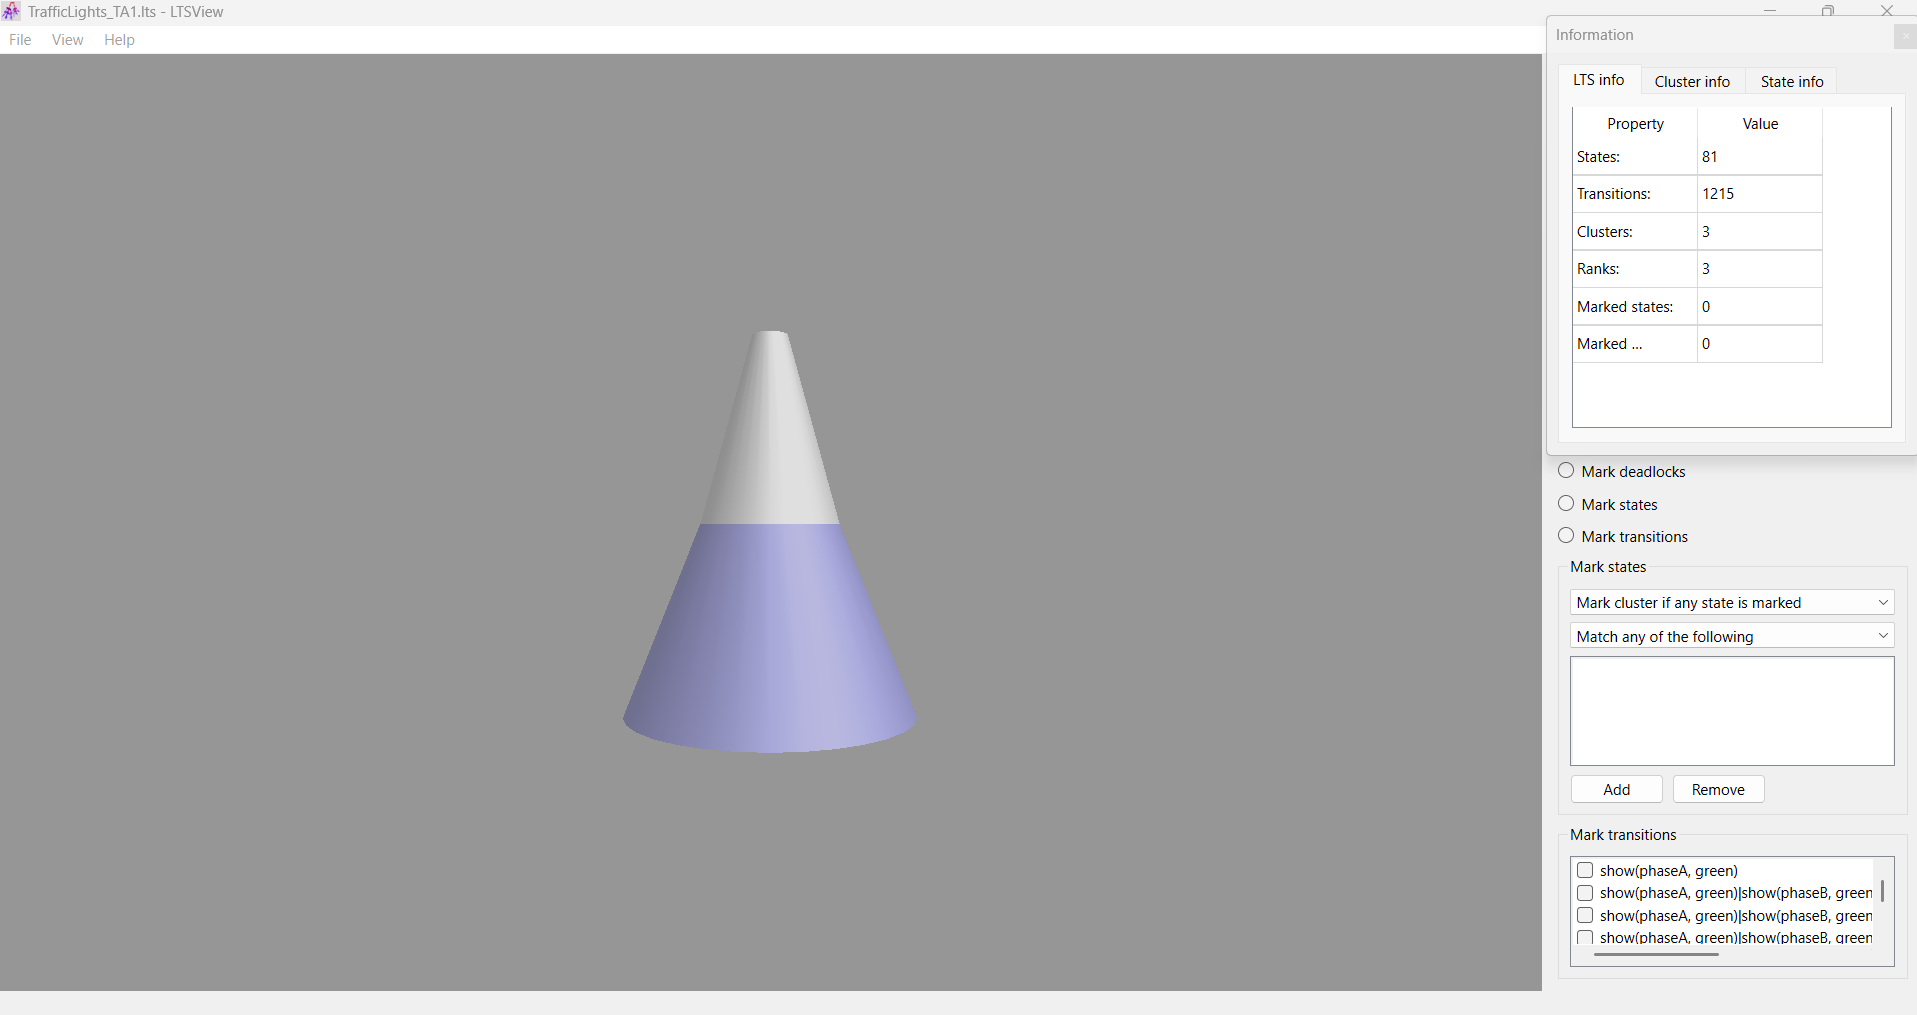
\includegraphics[width=1.0\textwidth]{ItsView Bilder zu 2b1-4/TA1StatesAndTransitions.png}
    \caption{LtsView Ansicht der Lösung zu Teilaufgabe 1}
    \label{fig:TA1}
\end{figure}

Vorgaben : 
(81 states, 1215 transitions)
 Referenzspezifikation: < 75 LOC


\subsection{2b.2}
Es ist anhand der in Abbildung \ref{fig:TA2RED} zu sehenden Darstellung der reduzierten Lösung über Ltsview zu erkennen, das die Lösung die Eigenschaften der Vorgaben erfüllt. 


\begin{figure}[H]
    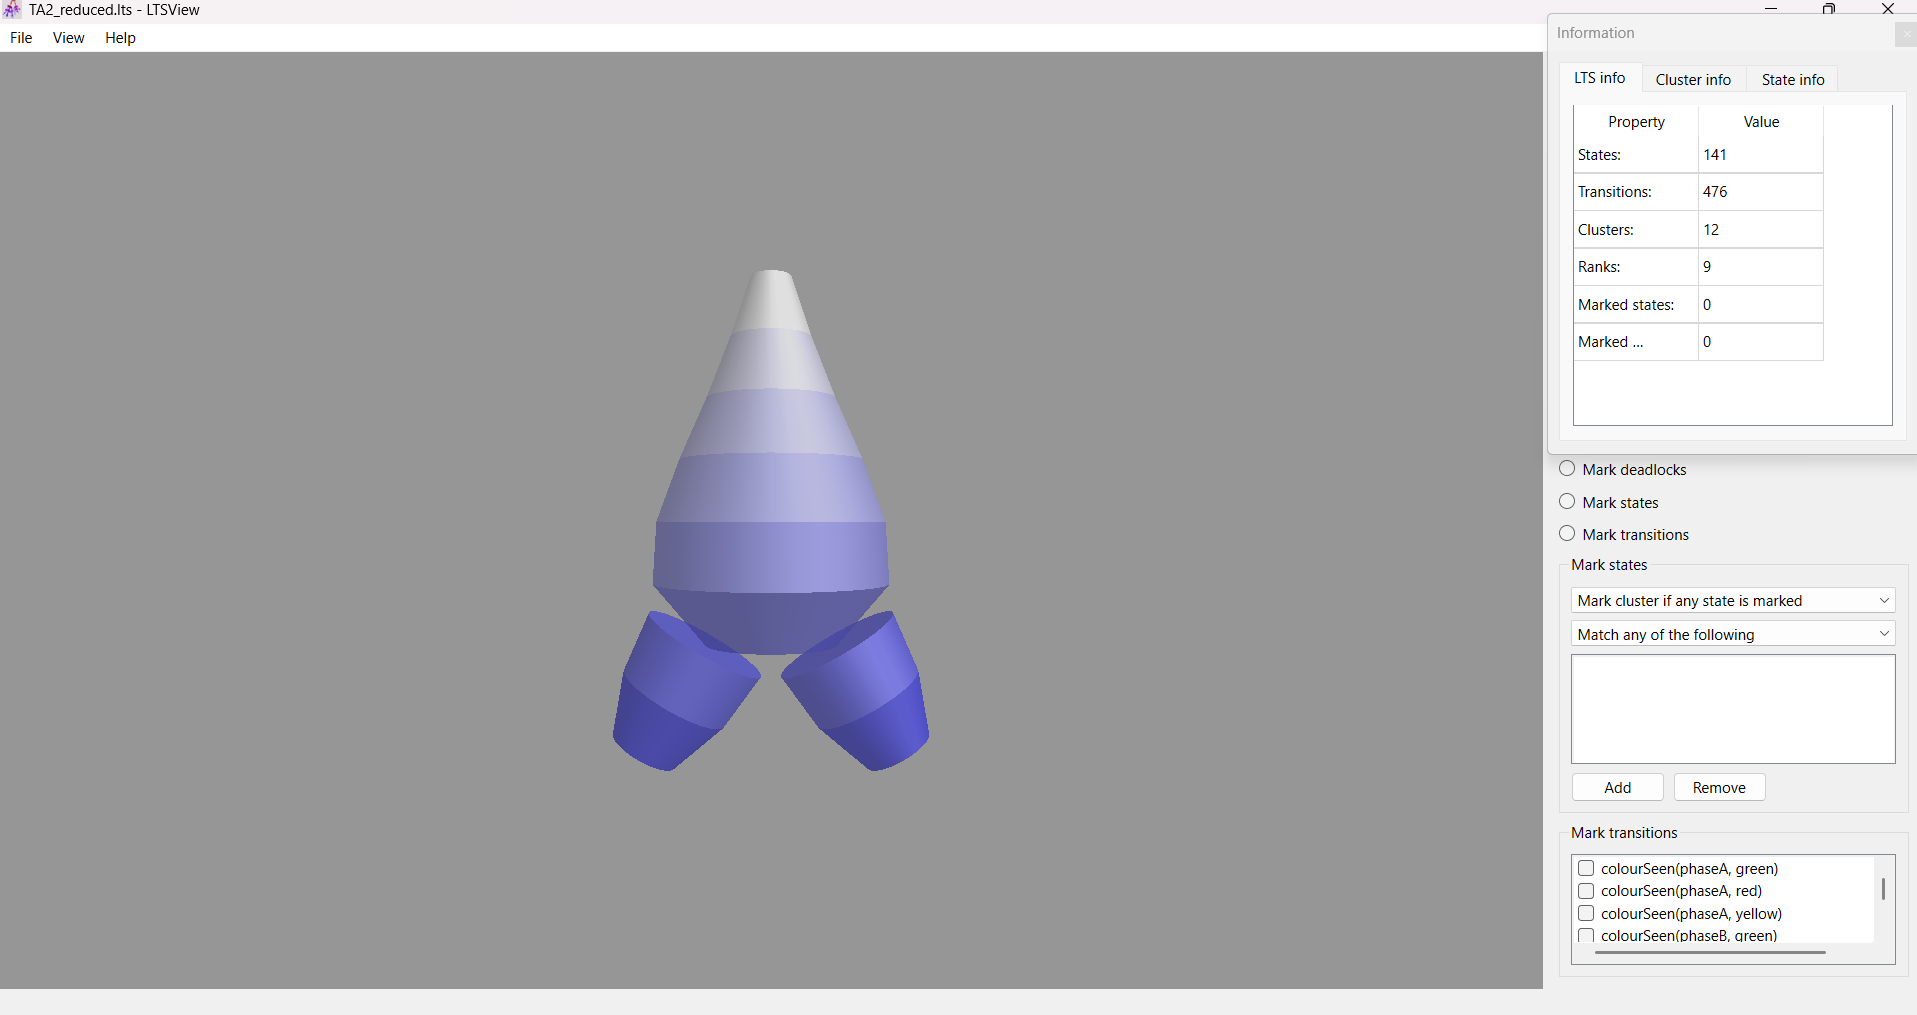
\includegraphics[width=1.0\textwidth]{ItsView Bilder zu 2b1-4/TA2ReducedS&T.png}
    \caption{LtsView Ansicht der Lösung zu Teilaufgabe 2}
    \label{fig:TA2RED}
\end{figure}

Vorgaben :
 (141 states, 476 transitions für die bbsim-reduzierte Version)
 Referenzspezifikation: < 130 LOC



\subsection{2b.3}
Es ist anhand der in Abbildung \ref{fig:TA3RED} zu sehenden Darstellung der reduzierten Lösung über Ltsview zu erkennen, das die Lösung die Eigenschaften der Vorgaben erfüllt. 

\begin{figure}[H]
    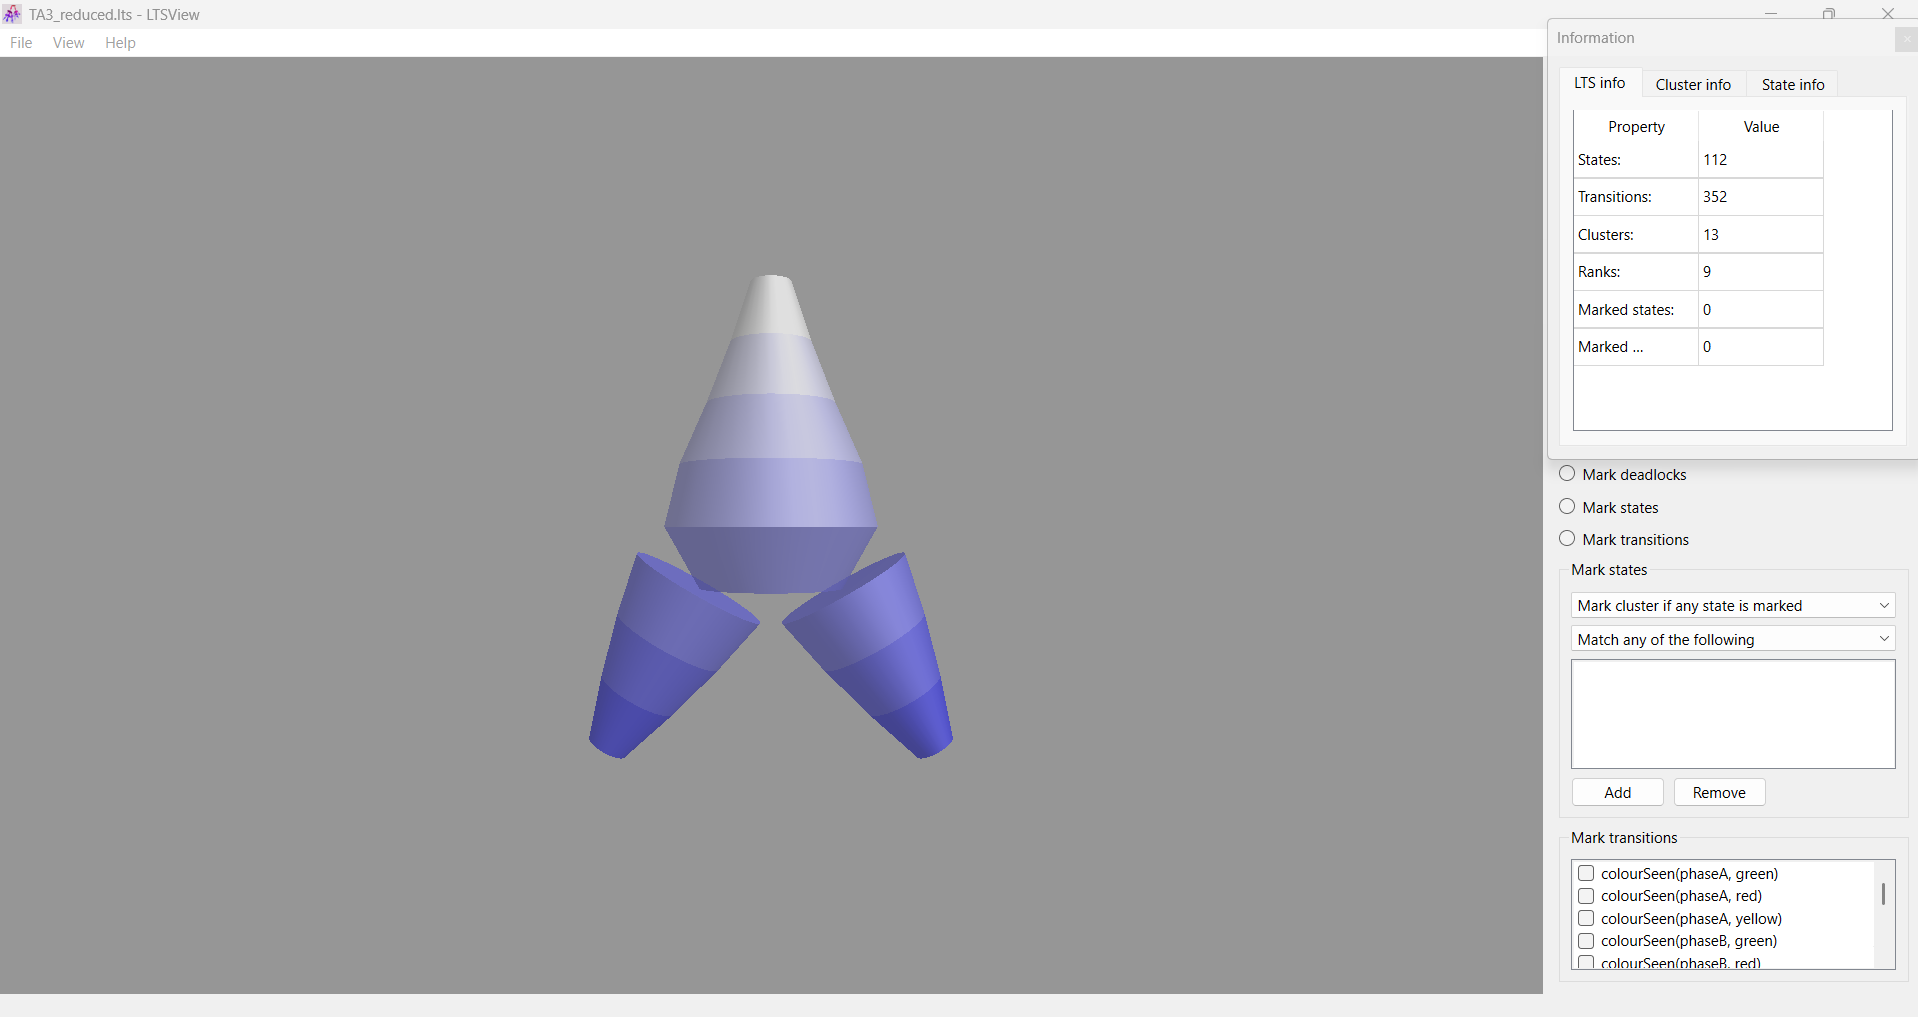
\includegraphics[width=1.0\textwidth]{ItsView Bilder zu 2b1-4/TA3RedS&T.png}
    \caption{LtsView Ansicht der Lösung zu Teilaufgabe 3}
    \label{fig:TA3RED}
\end{figure}

Vorgaben :
 (112 states, 352 transitions für die bbsim-reduzierte Version)
 Referenzspezifikation: < 130 LOC



\subsection{2b.4}
Es ist anhand der in Abbildung \ref{fig:TA4RED} zu sehenden Darstellung der reduzierten Lösung über Ltsview zu erkennen, das die Lösung die Eigenschaften der Vorgaben erfüllt. 

\begin{figure}[H]
    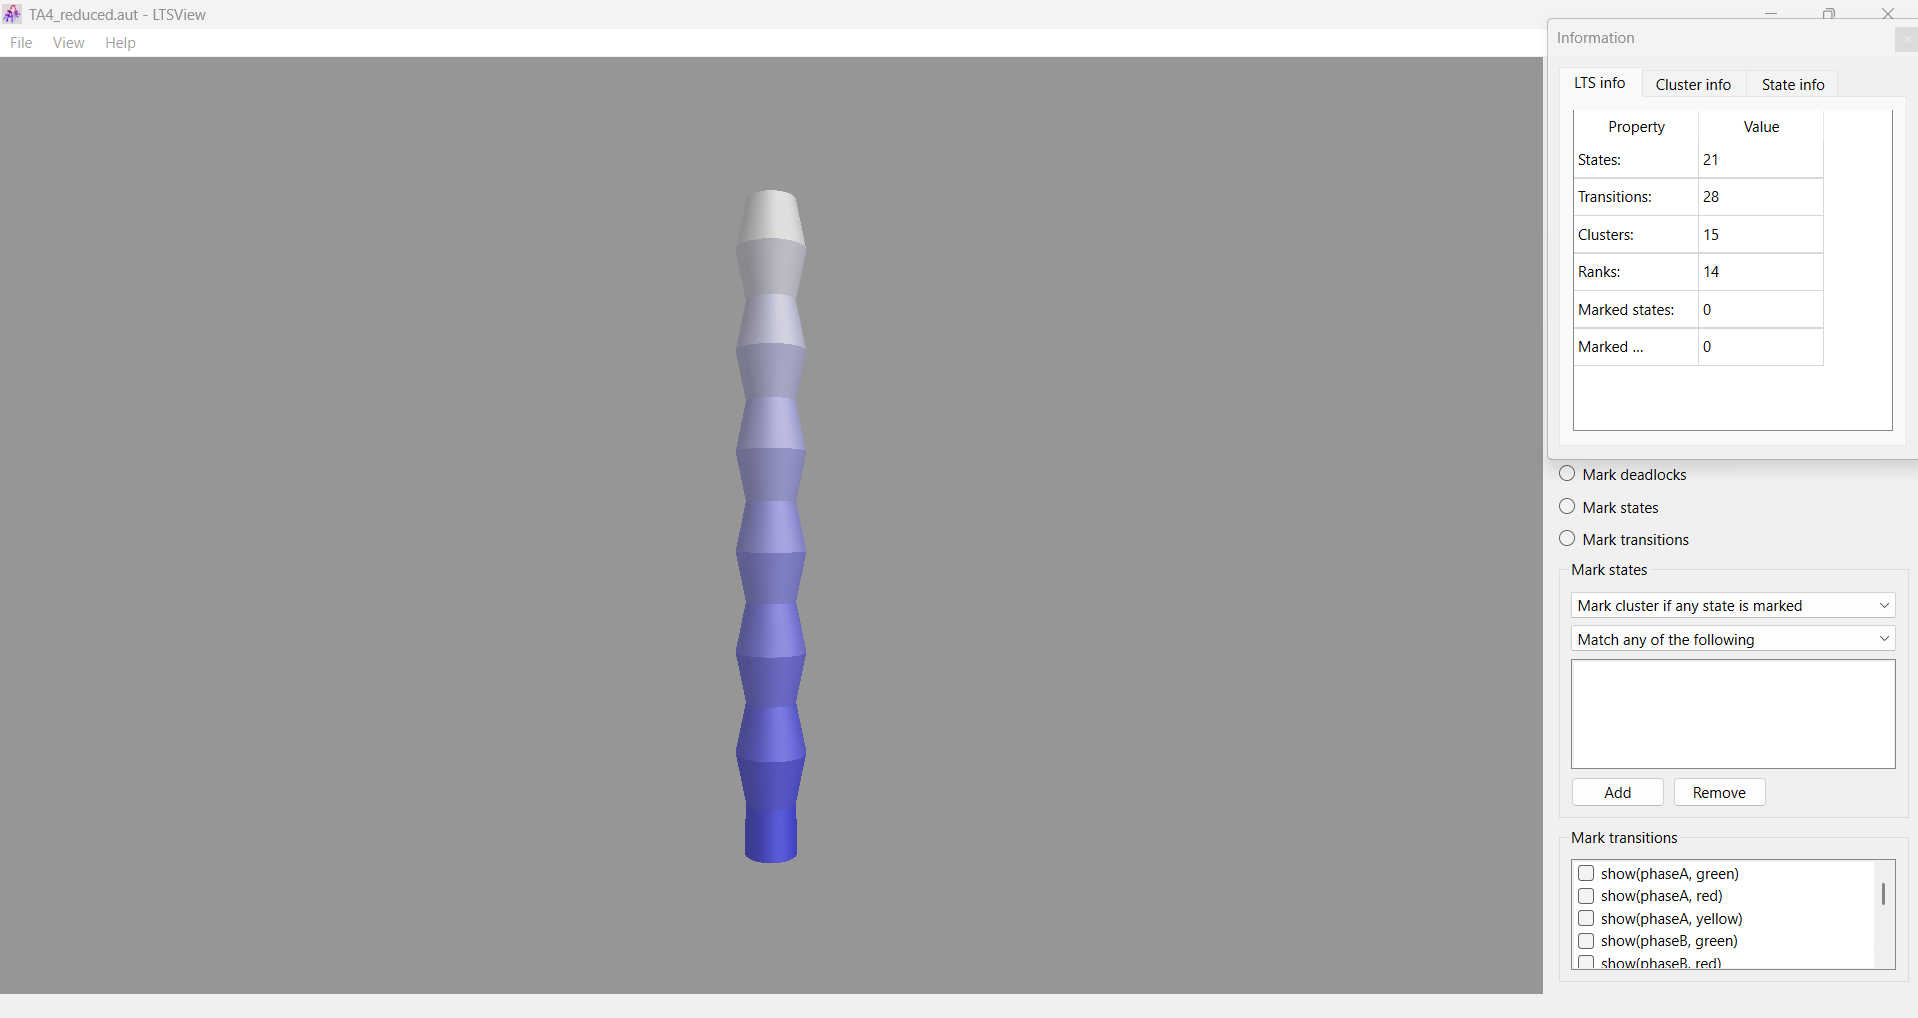
\includegraphics[width=1.0\textwidth]{ItsView Bilder zu 2b1-4/TA4RedS&T.png}
    \caption{LtsView Ansicht der Lösung zu Teilaufgabe 4}
    \label{fig:TA4RED}
\end{figure}

Vorgaben :
(21 states, 28 transitions für die bbsim-reduzierte Version)
 Referenzspezifikation: < 95 LOC


 \subsection{Vergleich mit der Musterlösung über ltscompare}

 Über den Konsolenbefehl welcher in Abbildung \ref{fig:vglcmd} genutzt wird lässt sich ein vergleich zwischen unseren und den Musterlösungen durchführen.
 An der Ausgabe ist erkennbar, dass alle vier durchgeführten Vergleiche erfolgreich abgeschlossen wurden. Die Ausgabe „LTSs are equal“ sowie der Rückgabewert „true“ bestätigen für jeden Fall, dass unsere Implementierungen unter Berücksichtigung der branching bisimilarity (basierend auf dem $O(m \log n)$ Algorithmus nach Jansen/Groote/Keiren/Wijs 2019) strukturell äquivalent zu den jeweiligen Musterlösungen sind.
 
 
 \begin{figure}[H]
    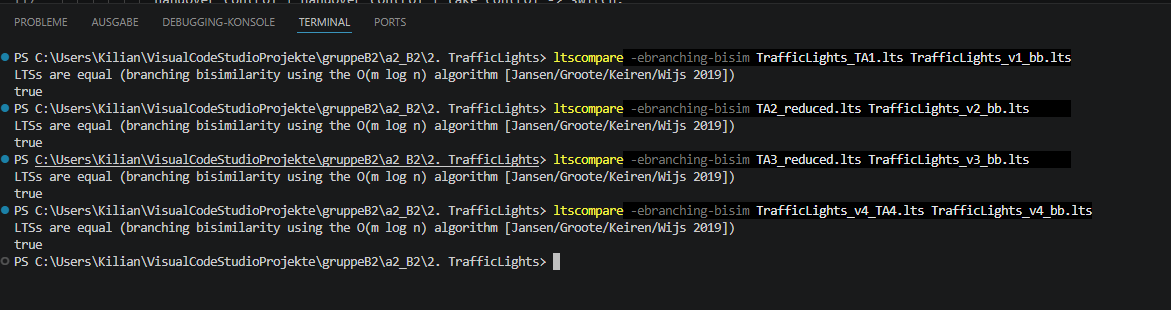
\includegraphics[width=1.0\textwidth]{Vergleichsbilder/Kommandozeilenvergleich1-4.png}
    \label{fig:vglcmd}
    \caption{Konsolenausgabe des Vergleiches unserer mit den Musterlösungen}
 \end{figure}



\end{document}

